\documentclass{article}
\usepackage[utf8]{inputenc}
\usepackage[english]{babel}
\usepackage{amsmath}% http://ctan.org/pkg/amsmath
\usepackage{listings}
\usepackage{graphicx}
\usepackage{comment}
\usepackage{float}
\usepackage{biblatex}
\usepackage{lscape}
\usepackage{csquotes}
\usepackage{multirow}
\usepackage{ragged2e}
\usepackage{tabularx}
\usepackage{xcolor}
\addbibresource{bibliography.bib}
\usepackage[a4paper,pdftex,bottom=20mm, width=160mm]{geometry} % A4paper margins
\setlength{\parindent}{0pt} % Tar bort indenteringen på paragrafer 
\setlength{\parskip}{1em}


\title{
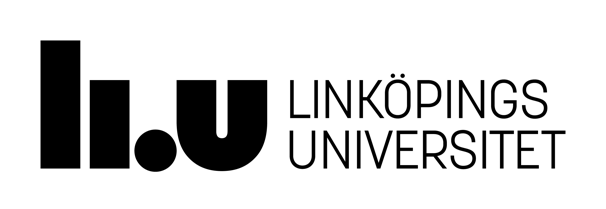
\includegraphics[scale=1.5]{liu_logga.png} \\
\vspace{2.0cm} \textbf{Testing Plan} \\
 \endgraf\rule{\textwidth}{.4pt}
  \large \textbf{TDDC88 Programutvecklingsmetodik}\\
   }
   
   
\author{Author: Company 3 - Testing Group \\ \\
    Document Owner: Anton Hänström, Test Leader}
\date{\today}

\begin{document}

\maketitle
\newpage
```latex
\section{Document Change History}

\begin{center}
\small\textit{Note: This change history table was generated by Autoleaf AI under the supervision of the Technical Writer. Only the most significant changes are highlighted, check the readme.md, found in gitlab, for more detailed information.}

\vspace{0.5cm}

\begin{tabular}{|p{0.05\textwidth}|p{0.09\textwidth}|p{0.17\textwidth}|p{0.14\textwidth}|p{0.39\textwidth}|}
\hline
\textbf{Ver.} & \textbf{Date} & \textbf{Modified Areas} & \textbf{Changed By} & \textbf{Description of Changes} \\
\hline
2.2 & 2024-10-17 & Req. Struct., User Classes, Func. Req., Non-Func. Req., Design Constraints & Analyst Team & Restructure document for clarity and traceability, introduce sub-requirements linked to main requirements, rename and restructure user roles section. Remove Software System Attributes section. \\
\hline
2.1 & 2024-10-10 & User Stories, Scope, Non-Func. Req., Overall Desc. & Analyst Team & Restructure user stories, clarify scope, streamline non-functional requirement descriptions, and improve overall description clarity. \\
\hline
2.0 & 2024-10-03 & Software Sys. Attr., User Stories, Constraints, Assumptions, Func. Req., Perf. Req. & Analyst Team & Introduce software system attributes, refine user stories, expand constraints, clarify assumptions, and provide specific details for functional and performance requirements. \\
\hline
1.1 & 2024-09-24 & Intro, Overall Desc., Specific Req. & Analyst Team & Expand initial structure with detailed descriptions of user roles, system functionalities, requirements, and constraints. \\
\hline
1.0 & 2024-09-19 & Intro, Overall Desc., Specific Req., Supporting Info & Analyst Team & Establish initial structure and content of the Requirements Specification document. \\
\hline
\end{tabular}
\end{center}

\vspace{1cm}
```
 

\newpage
\tableofcontents
\newpage




\section{Introduction}

\subsection{In Scope}

These are the main components the following Testplan has been centered around
\newline
\newline - Qualitative usability : The customers main focus is qualitative usability, which can be boiled down to a prioritization on qualitative interfaces and other components impacting usability, rather than delivering a large amount of mediocre components. 
\newline- Different levels of testing : The testplan will state, as clearly as possible, which levels of testing will be performed and furthermore how these levels of testing will be performed. 
\subsection{Out of Scope}
The following components will not be a centre piece of the Testplan
\newline
\newline- Main aspects outside of the scope : Aspects such as security testing and backend testing, while still being important, will not be the main focus of the project and therefore not the main focus of the testing plan. 
\newline - Quality of the code : Furthermore, while qualitative indentation and naming is very good, is will not be tested since it does not affect the usability of the product as much.

\section{Test Process}
\subsection{Workflow}
In large projects, a well structured workflow is essential for performing an organizing tasks in an efficient way. This section outlines the workflow for testing and the workflow for executing and evaluating test cases. The testing will be divided into stages to track the process in the workflow. \newline

Before initiating the workflow,it is important to define and make sure the rolls for testing are clear. This ensures tasks and responsibilities are divided and it is clear who will do what to prevent overlap in work. \newline

Then the first stage of testing is understanding the project requirements. This step is crucial for developing the test cases and must be done in collaboration with analysts. Once the requirements are defined and have been properly understood, the process will continue to the next stage, developing a testing strategy. This involves determining what types of tests will be performed, scheduling the execution and layout of the testing process. \newline

Next, the testing moves to creating test cases for the selected testing methods. This involves writing a thorough script for the test and describing how the test will be executed. Right before executing the test, the testing environment has to be set up. This will vary depending on what type of test it is but this involves setting up necessary tools and resources. \newline

The setting up of an testing enviroment will have the following workflow. Firstly, the environment requirments are defined, meaning getting an understanding of what is needed based on the test type. After that, allocating resources is important, which could be allocating and configuring the necessary servers or cameras, also configuring any testing tools that could be used. Lastly, validate and document the test enviroment for analysis and recreation of the test.\newline

Once the environment is ready for testing the tests are executed. This process is done in different ways depending on the type of test. For instance, acceptance tests will be performed together with customers, user tests involving external participants and automated tests will run without monitoring. \newline

After tests are complete, the final stage is reviewing results and addressing bugs and issues. This includes determining if requirements must be retested or if they can be labeled as achieved. 




\subsection{Bug Handling Process}
\subsubsection{Selected bug tracking tool} 
Bugs will be tracked using the Microsoft Planner tool. This will be a way to track unexpected problems that come up in the project and have a way of managing them efficiently. This tool will be used to label the incidents in how important they are and in what order they will be handled. This is a way of tracking that will be efficient for development since Microsoft tools are used for more parts in the project. 


\subsubsection{Process for reporting, prioritizing, and assigning bugs}
The way that bugs will be reported is by creating an incident in Microsoft planner. After this is created the bug will be labeled by the creator on how important it is and how it should be prioritized. With Microsoft planner the team can create different boards for different types of bugs or label as severity. After this, for efficient communication, the scrum meetings will be used to discuss these incidents and who will be responsible for the resolution of the bug. This way every developer will have knowledge of the bug and a resolution can be discussed with the entire group. If bugs are not solved properly or other developers are not aware of the issue then that can cause more issues and unnecessary work.


\subsubsection{Workflow for bug resolution and verification}
The bug resolution will be solved in different ways depending on the issue, the developer, together with the team, will come up with a solution and the code will be fixed if it is possible. After debugging, the member will merge the fixed code with the old code. The incident in Microsoft planner will be closed. The other developers can after that continue with their work in that code without being affected by the incident. The lead developer is responsible for delegating and taking the final decision if the bug will be resolved or not and if who will fix it. If a bug cannot be solved then that will be noted to the entire team and actions will be taken 


\subsubsection{Metrics for tracking bug trends and resolution efficiency}
Tracking bug trends will be done manually from the incidents created in Microsoft planner when or if there is something that needs tracking. The aim for the project is that the debugging is done thoroughly so that there are no trends in bugs to track. If needed,  the tracking of trends will be done in excel. The Microsoft planner board that need analysis and tracking of trends will be exported into excel. There the developers can see trends in metrics and analyze the data. 


\subsubsection{Bug tracking for continuous improvement}
Bug tracking is important for continuous improvements as this allows the team of developers to see and understand the issues that has been raised and how they have been resolved. This means that if this issue comes up again there will be a quick resolution, but perhaps the issue will never come up again as the team knows what to avoid. The bug tracking enforces this when the group of developers discuss this during the scrum-meetings and have this communications on bugs and debugging.


\subsection{Traceability}
The plan is to implement traceability in two key ways to ensure that all tests are directly linked to the corresponding requirements and user stories, providing a clear understanding of which features have been verified.

\subsubsection{Requirement-to-Test Traceability} Each requirement defined in the project will be linked to a specific test or set of tests. This ensures that every requirement is accounted for and tested through a structured process. For example, when a test is executed, it will be easy to trace back to which requirement the test is verifying. Additionally, each requirement will be associated with a relevant user story, ensuring that the user perspective is always kept in focus during the testing process.

\subsubsection{Test Traceability Matrix} To effectively manage and track the testing process, we will use a Test Traceability Matrix. This matrix will provide a comprehensive overview of all tests, showing the following details:

\begin{itemize}
    \item Which tests have been performed.
    \item When the tests were executed.
    \item Whether each test passed or failed.
    \item Which requirement each test covers.
\end{itemize}

By using this matrix, we will have a clear view of testing progress and be able to easily identify any missing or untested requirements. Additionally, it helps ensure that any failed tests are properly addressed, preventing gaps in coverage. This approach provides both clarity and accountability throughout the testing phase, ensuring continuous improvement and alignment with the project’s goals. \\

For automated tests, the \textit{Test Traceability Matrix} will not be updated every time they are run. Instead, it will only be updated when there is a change in the outcome. For example, if an automated test has been consistently successful but suddenly fails, the \textit{Test Traceability Matrix} will be updated at that point. This ensures that the matrix reflects significant changes in the testing results, avoiding unnecessary updates while still maintaining an accurate record of test performance.


\section{Unit Testing}

During the sprints, the code—divided into 4 sections—will need to be tested to ensure continuous integration, primarily focusing on each section separately, with system tests being conducted less frequently. The four different sections that the code is written in are LAN and External, both written in python, ACAP, written in C, and Client, written in JavaScript xml. All sections except the client will be tested through unit testing. The client part will tested as a whole while executing user tests.


\subsection{Tools}
Given that the code is segmented, each section requires its own set of unit tests. By utilizing an xUnit-based framework (such as JUnit or pytest), we can maintain a consistent and structured method for testing each code segment. For the code in python, LAN and external, we will use pytest. This is a python tool for testing and will be used together with the pipeline in Git to create automated tests. The same will be created for the ACAP section together with cunit tests cases. Git pipeline will be used to create automated tests. The deployment team will create a pipeline in Git that will be utilized by testers for the creation of automated tests. 

\subsection{Workflow}
The way unit testing will be created and executed will be both manual and automated testing. The thing that will be created first is the pipeline, this, as mentioned previously, will be created by the deployment team. Then the different test cases will be created for each section at a time until all functions in the code have been tested. This will be run manually first by running each individual test case as a way to check that the tests are done and no error exists. When all test cases have been checked and have passed the code the files will run via the pipeline to avoid manual testing. When the test cases have been added so they run on the pipeline the developers will not be able to merge files unless the testing stage is executed successfully. The unit tests are written on each segment alone and tested without other parts of the system, this is because of isolation. When they are tested as independently as they can it will be easier to spot the error if the testing stage is unsuccessful while pushing. The needed functions and classes will be mocked to generate isolated testing. 

\subsection{Automated vs Manual testing }
In unit testing both automated and manual testing will be used. They both have their own function and how unit tests will use manual tests will be for testing the test case. Before uploading in the pipeline the tests need to be working correctly so that the pipeline only executes test that work with the code. The manual tests will be run by themselves in the terminal and when correctly executed they will be uploaded to the pipeline. Automated tests will be used for all developers to have a backup check that all functions still work before they push to the branch in git. If this had to be done manually then it could become a time issue and might be skipped. Having automated tests ensures that only working code is merged into the branch and all possible issues stays on the local code. This can be a check for developers to use instead of checking all code works, the testing stage will tell them what file and what test failed so that the developer knows where the issue lies. Creating unit tests will automate the testing process early on, freeing up time later and providing a continuous and clear understanding of how the code development is progressing. Additionally, since there are more developers than testers in the company, this automated framework will streamline the workflow and help manage the volume of tests efficiently. Automated test will only be performed for unit testing while manual tests will be used for the other types of tests. 

\section{System Testing}
System testing tests the entire system when the four components are put together. This involves testing the different parts of the project to make sure it all works together. Together with unit testing we can make sure all components work and that the entire integrated system works . The system tests will be performed using functional testing and non-functional testing. The system tests will be executed as a way to control requirements to see that the entire integrated system aligns with these.  System testing will be used to ensure there is a deliverable system at the end of each sprint, therefor these tests will be spread out during the project.
\subsection{End-to-End or E2E testing}

One part of the system testing will be E2E testing. The aim is testing the workflow from beginning all the way to the end. The goal is finding the critical path for the relation between two or more of the components and then test this path in one go. 

The start of the E2E testing is understanding the critical path, what functions are co-operating and how well? After that the E2E test in constructed, mainly manual test since big E2E test are time consuming to create and time is one of the most scares resources in this project. The E2E tests will be created in the same way as the test cases and executed according to the test plan workflow. The test cases is linked to a certain amount of requirements, and the E2E will then be a amount of test cases that shall be executed after one another. In that way the E2E can be linked to the requirement traceability matrix. 





\section{User Experience (UX) Test}

\subsection{Objectives}
The primary goals of UX testing are:
\begin{itemize}
    \item To assess the ease of use, efficiency, and satisfaction with the system from a user perspective.
    \item To identify potential areas for improvement in functionality, aesthetics, and user engagement.
    \item To deliver actionable insights to developers for system refinement between iterations.
\end{itemize}

\subsection{Test Setup}
\textbf{Role-Based Scenarios:} Test subjects will receive a role description (e.g., guard) and will be given a series of tasks to complete relevant to that role. Each task is aligned with a specific use case to ensure coverage of different functionalities and user flows.

\textbf{Metrics Captured:}
We will monitor and record:
\begin{itemize}
    \item \textbf{Number of clicks:} Helps gauge efficiency in completing tasks.
    \item \textbf{Time to complete tasks:} Measures how intuitive and fast the system is for users.
    \item \textbf{Task success rate:} Indicates task completion and user understanding.
\end{itemize}


\subsection{Post Test Questionnaire}

Upon task completion, test subjects will complete a questionnaire designed to gather feedback on:
\begin{itemize}
    \item \textbf{Usability:} Was the system easy to navigate and understand?
    \item \textbf{Confusion Points:} Did they feel confused at any stage? If so, where?
    \item \textbf{Professional Impression:} Does the system appear polished and professional?
    \item \textbf{Aesthetics and Functionality Feedback:} Is there anything they would change or improve visually or functionally?
\end{itemize}

To quantify usability, the \textbf{System Usability Scale (SUS)} will be utilized as part of the questionnaire.

\subsection{Test Subjects}
To ensure diverse perspectives:
\begin{itemize}
    \item Test subjects will be selected from outside the company.
    \item Participants will have varied technical backgrounds and levels of expertise to reflect a range of user experiences.
\end{itemize}

\subsection{Testing Schedule}
Testing will commence in \textbf{Iteration 3}, aiming to begin as soon as there is sufficient functionality. The early testing will allow us to gather insights for developers to improve the system iteratively.

A follow-up UX test will be conducted in \textbf{Iteration 4} to track improvements and validate enhancements based on initial feedback.



\section{Testing External Libraries}
Throughout the development process, it is essential to ensure that all external libraries integrated into the application are properly tested. These libraries, such as those handling JSON parsing (e.g., "jansson"), must be validated to guarantee they perform their intended functions correctly within the system.\\

Testing of external libraries will be conducted continuously as new libraries are introduced. This approach ensures that any potential issues are identified and resolved early. Close collaboration with the developers will be maintained to verify that each external component integrates seamlessly with the application and meets the required standards for functionality and reliability.


\section{Acceptance Test}
An acceptance test is conducted to determine whether a system or product meets Axis' specifications and is ready for delivery. These tests will be held after each prototype stage, following unit, integration, and system testing.


\subsection{Acceptance Test Process}
We plan to implement structured development cycles, where an acceptance test will be conducted after each prototype stage. These tests will focus on evaluating the features that have been completed during the cycle. The primary objective of the acceptance test is to gather detailed feedback from Axis, ensuring that the product is progressing in line with their specifications and expectations. By continuously validating the development with Axis, we aim to ensure that any necessary adjustments are made early, facilitating smoother progress towards the final product.


\subsubsection{Execution Plan for Acceptance Test}
In the later stages of each development cycle, the testing team within the company will conduct internal tests. The primary objective is to evaluate the product from a customer perspective, assessing which user stories have been completed and identifying functionalities that are still under development. Based on these findings, the testing team will create an acceptance test designed to present Axis with a user-centric view of the application's current capabilities. Axis will then provide feedback on how our solutions align with the established requirements, offering insights that we will relay to the developers to guide further improvements.

\textbf{Option 1: Live, face to face meeting}\\
This option could be defined as the booking of a certain amount of meetings, where the customer will have the chance to get hands-on experience with the application and go through a variety of pre-set tasks, with the chance of questioning and feedback. The pros of this option is the level of understanding a customer actually gets from hands-on experience, along with the change of immediate feedback and discussion, which could be very valuable. The cons of this option is of course the amount of time this option actually takes, having to book and go through with a physical meeting.

\textbf{Option 2: Digital meeting}\\
Option 2 is having digital meetings where a tester in the company will be live with the system to show the user. The user test will be performed similarly to if the test was live, but this will be more of a visual walkthrough of the system and the features. Axis will here have the possibility to leave their feedback and comments on what they like and what they do not like. However, if this option is chosen then there will possibly be a decrease in performance as the computer will have to work harder. Showing the system live or in video will not create the same issue. The tester at axis will not have the ability to test and play around with the system, therefore only seeing the parts of the system that the tester from Company 3 shows them. This can be an efficient way in testing as there will be no time spent for the customer to have to learn the system and the time will be well spent. 

\textcolor{gray}{\textbf{Option 3: Over email, videos, pictures, and text [OBSOLETE]}\\
This option could be described as the sending of pictures and videos of testing of the application, with the aim to show the results of functionality and usability of the application at that certain time. The pros of this option is the resource management aspect, since qualitative requirements and testing should ensure that each iteration will produce a qualitative product. The cons of this option is of course that the customer will have little hands-on experience with the application, which could present hidden defects a video or picture could not. }

\textbf{Axis decision} \\
Axis has decided to proceed with a combination of face-to-face and digital meetings for the acceptance test. They believe that these options will provide a more comprehensive evaluation of the product, allowing for hands-on experience and detailed feedback. However, they have opted not to use email, videos, or pictures, as these methods may not provide sufficient insight into the system’s usability and functionality.


\section{Time Plan}

The testing process will follow the project’s structured development cycles, with each cycle concluding with an acceptance test. There will be four iterations, each designed to refine the system and ensure that it meets the required specifications from Axis. 

\subsection{Iteration 1}
\textbf{Duration:} Week 40 - Week 41\\
\textbf{Focus:} Finishing the Version 1 of the Quality Assurance plan that the Testers are responsible for. Starting creating tests to cover the requirements, creating the structure for how these tests will like. Rough draft of the testing plan, what parts should the test plan contain, focusing on the acceptance test and unit testing since this will be what is testable at this stage. Gaining technical knowledge in how automated tests can be done.\\
\textbf{Acceptance Test:} Conducted Thursday Week 42.

\subsection{Iteration 2}
\textbf{Duration:} Week 42 - Week 45 \\
\textbf{Focus:} Fixing the Test Plan in accordance to feedback, completing version 2 of the Test Plan. Starting the implementation automated tests in unit testing. First draft of system testing as well as researching what structure the UX tests will have. \\
\textbf{Acceptance Test:} Conducted Thursday Week 46.

\subsection{Iteration 3}
\textbf{Duration:} Week 46 - Week 47\\
\textbf{Focus:} Complete the instructions for the first user experience tests. Starting with user experience testing. Gaining input from users that gets passed along to the developers and management team. \\
\textbf{Acceptance Test:} Conducted during Week 48.

\subsection{Iteration 4}
\textbf{Duration:} Week 48 - Week 49\\
\textbf{Focus:} Final user experience testing ensuring as few bugs as possible are prescient and that we have the best possible product. Axis will have the opportunity to conduct UX testes if they are interested in this stage to gather even more feedback.  \\
\textbf{Acceptance Test:} Conducted during Week 50.

\subsection{Special Considerations}

\textbf{Post-Exam Push}: Due to high workload during the first study period (Study Period 1), we anticipate dedicating additional resources to finalizing the test plan and completing remaining tests directly after the exam season. This is planned for Week 2 (Study Period 2), where the team will have more available time to focus on testing tasks.

\subsection{Summary of Milestones}
\begin{itemize}
    \item \textbf{Week 42}: First acceptance test
    \item \textbf{Week 46}: Second acceptance test
    \item \textbf{Week 48}: Third acceptance test
    \item \textbf{Week 50}: Final acceptance test and test plan completion
\end{itemize}

\section{Risk Assessment}
It is important to identify and mitigate risks that may affect the success of the testing process. Below are some potential risks that have been identified:

\textbf{Limited Time in Study Period 1}\\
Due to a heavy academic workload during Study Period 1, the team has limited time to dedicate to this project. This constraint could lead to delays in the completion of tests and documentation. To mitigate this, we have planned a \textbf{Post-Exam Push} in Week 2 of Study Period 2, where additional resources will be allocated to finalize any remaining tasks, including testing and bug fixing.\\
\textbf{Probability: 4, Impact: 4, Risk Factor: 16}


\textbf{Not Enough Time to Complete the Last Stages of Testing, System and User Experience Testing}\\
If time constraints prevent the completion of the final stages of testing, such as system and user experience testing, there could be undetected usability issues in the application. To reduce this risk, we aim to start system testing in iteration 3 and 4.\\
\textbf{Probability: 2, Impact: 5, Risk Factor: 10}

\textbf{Technical Knowledge for Automated Testing}\\
Another risk is the need for the team to acquire sufficient technical knowledge to implement automated testing in the Git pipeline. As automated testing is an integral part of our development process, any delays in learning or implementation could affect the consistency and reliability of our testing framework. To mitigate this, we will prioritize learning this system early in the project and seek support from developers to ensure we are prepared to use the Git pipeline effectively for automated testing.\\
\textbf{Probability: 3, Impact: 3, Risk Factor: 9}

\textbf{Bad Communication with Developers Leading to Difficulties in Achieving Good Unit Testing}\\
Inadequate communication with developers could complicate unit testing efforts, which might affect our ability to monitor code quality closely. However, since the focus is on end-user experience rather than code quality, this risk has a lower impact. To address this, we will establish regular check-ins with the development team to make sure that the unit testing goes as planned.\\
\textbf{Probability: 2, Impact: 2, Risk Factor: 4}



\cite{tan2014introduction}

\newpage
\printbibliography

\end{document}
